In many real-world scenarios, one sensor and one source of information may not suffice. Sensors in general have specific technical specifications and limitations. For example, imagine a surveillance system tracking enemy troops. A raw image from a camera working in the visible spectrum may not capture information about people using camouflage, and therefore, tracking such targets with this camera alone becomes intractable. However, if we use additional information from an infrared camera, targets become clearly visible and combined measurements will have a higher signal-to-noise ratio. Techniques involving combining information from different sources are called information fusion. In this section, we will briefly describe the types of information fusion that exist and describe how this information can be used to get more accurate tracking results for the GM-PHD filter.

Information fusion, or information integration, is generally a broad term, mainly because sources of information differ a lot. For instance, \textit{data fusion} is the process of merging data from different data sources and in different formats to create a comprehensive picture of the environment \cite{kleinSensorDataFusion2004}. Data sources may refer to measurements from sensors, data from a database, or human input, while data types may include text, images, audio inputs, or binary data. On the other hand, \textit{decision fusion} refers to collecting decisions from different algorithms that may look at the problem from different perspectives or work with different data inputs, and combining these decisions to create one final decision. Ensembles of different machine learning algorithms, for example, for pattern prediction, are an example of decision fusion \cite{mangaiSurveyDecisionFusion2010}.

In this work, we will refer to another fusion technique called \textit{sensor fusion}. In principle, sensor fusion is a subset of data fusion, which involves collecting data from various sensors and merging it to get a more precise and complete estimate of the environment. The example from the introduction to this section is also an example of sensor fusion. There may be many different types of sensors, including cameras, radars, lidars, sonars, or infrared cameras. Every sensor measures different aspects of the tracked environment, and the combined information describes the surrounding world more precisely.

Regarding Bayesian inference and multi-target tracking, we create estimates of moving objects, and there are many variables that can input uncertainty: the detection rate of the sensor, the quality of the tracking algorithm and its implementation, the environment conditions where the sensor operates, etc. And while the algorithm may be replaced with the one providing better estimates for a specific problem, physical limitations of sensors and the environment cannot be addressed easily. For example, let us take the AN/MPQ-53 radar, which is a part of the Patriot system, a surface-to-air missile system used for air defense deployed in many countries. The exact technical specifications of the radar are far beyond the scope of this work. However, we will give an example of what may cause the radar to fail to detect targets.

The AN/MPQ-53 radar has a 120-degree field of view with a 170 km range \cite{wolffMPQ53Radartutorial}. However, there may be physical limitations of the environment that create blind and clutter zones. For instance, imagine the situation where the radar is deployed on a surface and is targeted to track air objects above the sea. The water may cause spontaneous reflections of the radar rays and cause clutter measurements. Moreover, the curvature of the terrain may create a blind zone so that the radar will not be able to track targets flying at low altitudes. This example is shown graphically in Figure \ref{fig:radar-blind}.

\begin{figure}[ht]
    \centering
    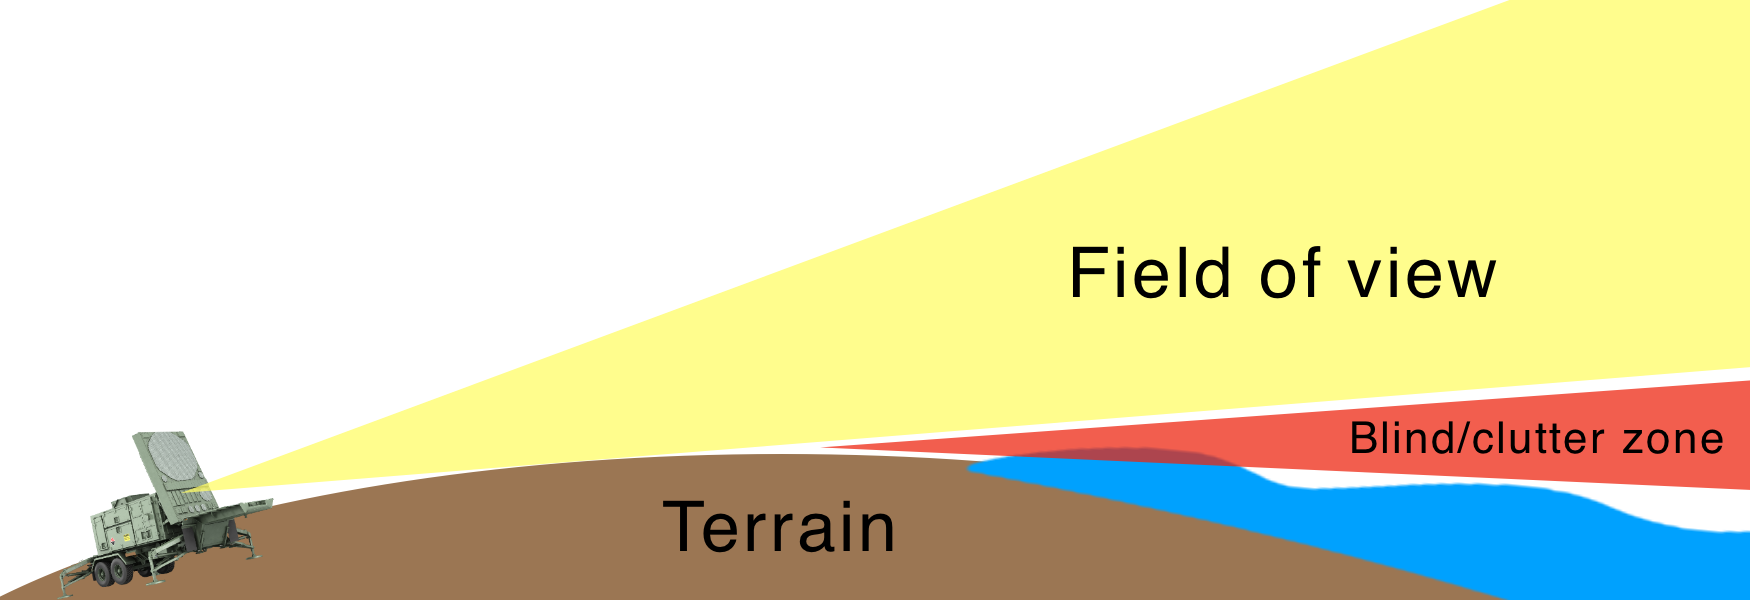
\includegraphics[width=.95\linewidth]{figures/radar-blind.png}
    \caption[Example of a radar blind zone caused by the curvature of the terrain and reflections from water surface.]{An example of the AN/MPQ-53 radar deployed on the surface with curvature and targeted at the sea. The curvature causes the blind zone, and reflections from the water surface may cause clutter measurements.}
    \label{fig:radar-blind}
\end{figure}

This problem may be addressed in several ways, one of which, that is covered in this work, is to use information fusion techniques. For example, we can incorporate additional information from other sensors placed after the curvature that supplements additional data about the blind zone and therefore covers the area that stays invisible to the radar. This source of additional information may be another radar or a different type of sensors, or even a soldier with binoculars. We can then input this additional information to the GM-PHD filter to improve the tracking performance. The example of such mitigation is illustrated in Figure \ref{fig:radar-additional-range}.

\begin{figure}[ht]
    \centering
    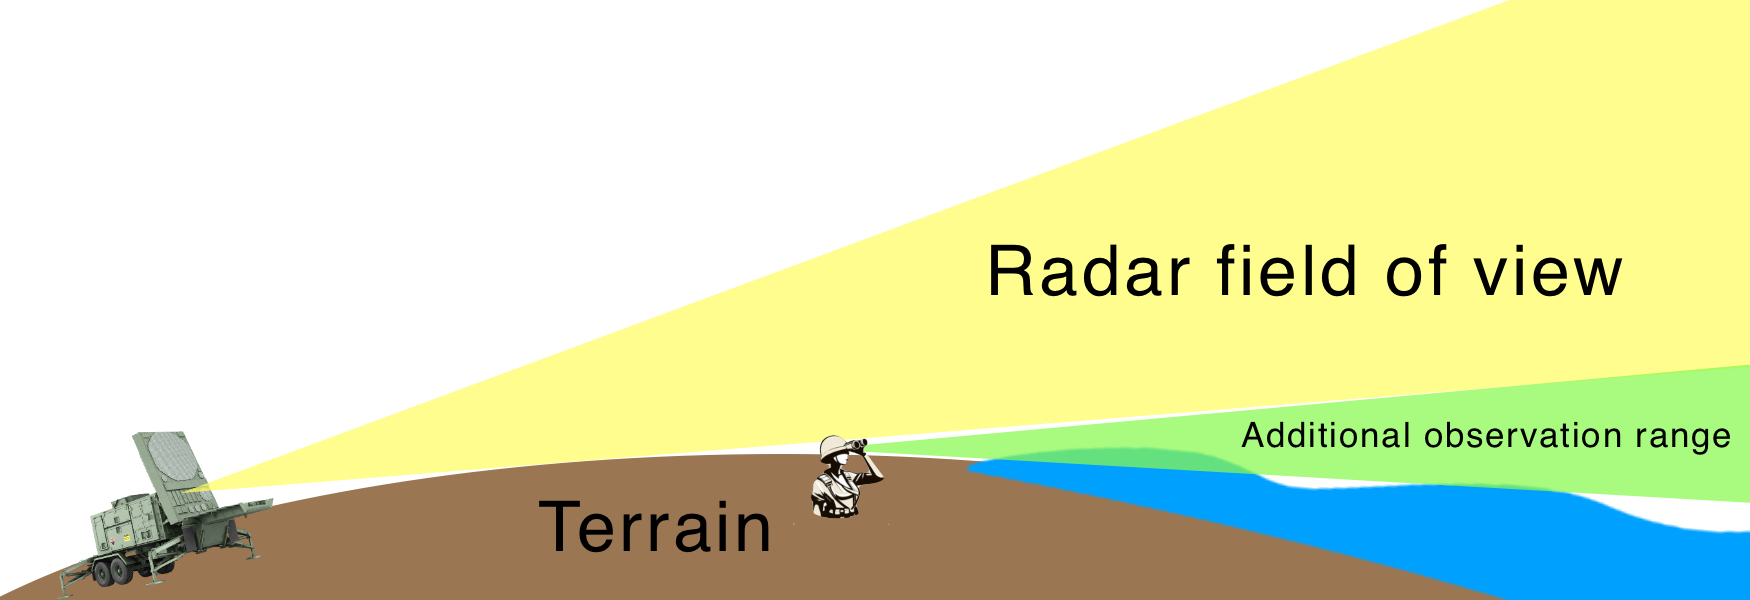
\includegraphics[width=.95\linewidth]{figures/radar-additional-range.png}
    \caption[Example of radar blind zone mitigated with additional observation range from soldier with binoculars.]{An example of the AN/MPQ-53 radar deployed on the surface with curvature and targeted at the sea. After the curvature, there is a soldier with binoculars with the additional observation range that covers the blind zone of the deployed radar.}
    \label{fig:radar-additional-range}
\end{figure}

We now define the imputation of additional data formally. Given that an instance of the GM-PHD filter with the CV model is running and at every time step $k$ it gets measurements from a sensor mixed with clutter in a set $Z_k$. Let there be an additional sensor that operates in the blind zone of the first radar. The second sensor measures position and velocity of targets $\vecat{m}{\psi}$ appearing in the blind zone with the uncertainty given by the covariance matrix $\vecat{P}{\psi}$ and the weight denoting the expected number of targets at this location, denoted $w_{\psi, k}$. Also, every such component is assigned with a unique tag $T_{\psi, k}$. All measurements of the second sensor create a set of additional states at time $k$, denoted $\Psi_{F, k} = \{ w_{\psi, k}^{(i)}, \svecat{m}{\psi}{(i)}, \vecat{P}{\psi}{(i)}, T_{\psi, k}^{(i)} \}_{i=1}^{J_{\psi, k}}$, where $J_{\psi, k}$ denotes the number of additional state estimates. Given that the dynamics of targets is Gaussian-linear, we propose that the intensity function of these additional measurements as $\psi_k(\mathbf{x})$, which is a Gaussian mixture of the following form:

\begin{equation}\label{eq:gm-phd-fusion-fusion-intensity}
    \psi_k(\mathbf{x}) = \sum_{i=1}^{J_{\psi, k}} w_{\psi, k}^{(i)}
        \mathscr{N}\left(\mathbf{x}; \vecat{m}{\psi, k}^{(i)}, \vecat{P}{\psi, k}^{(i)}\right).
\end{equation}

The GM-PHD filter is then modified to include additional information. We include this intensity in the prediction step of the GM-PHD filter, defined in Theorem \ref{theorem:gm-phd-prediction}, that will thus have the following form:

\begin{theorem}[The GM-PHD filter with external information prediction]\label{theorem:gm-phd-fusion-prediction}
    Given that assumptions from Section \ref{sec:gm-phd} apply and the posterior intensity of the previous time step $v_{k-1}(\vecat{x}{k-1} | Z_{1:k-1})$ is a Gaussian mixture of the form:

    \begin{equation}
        v_{k-1}(\vecat{x}{k-1} | Z_{1:k-1}) = \sum_{i=1}^{J_{k-1}}
        \mathscr{N}\left(\vecat{x}{k-1}; \vecat{m}{k-1}^{(i)}, \vecat{P}{k-1}^{(i)}\right),
    \end{equation}

    \noindent where every Gaussian component has a unique tag or label assigned to it, which forms the set of tags:

    \begin{equation}
        T_{k-1} = \{ T_{k-1}^{(1)}, \ldots, T_{k-1}^{(J_{k-1})} \}.
    \end{equation}

    \noindent Also, let additional state estimates from other sensors have the form $\Psi_{F, k} = \{ w_{\psi, k}^{(i)}, \svecat{m}{\psi}{(i)}, \svecat{P}{\psi}{(i)}, \allowbreak T_{\psi, k}^{(i)} \}_{i=1}^{J_{\psi, k}}$ and the fusion intensity is given by Equation \ref{eq:gm-phd-fusion-fusion-intensity}. Then the predicted intensity at time $k$ is also a Gaussian mixture, defined as:

    \begin{equation}
        v_{k|k-1}(\vecat{x}{k} | Z_{1:k-1}) = \gamma_k(\vecat{x}{k}) + \psi_k(\vecat{x}{k}) + v_{S, k|k-1}(\vecat{x}{k}),
    \end{equation}

    \noindent where $\gamma_k(\vecat{x}{k})$ is given in Equation \ref{eq:gm-phd-birth-gm} and $v_{S, k|k-1}(\vecat{x}{k})$ is the PHD function of survived targets given in Theorem \ref{theorem:gm-phd-prediction}. The set of tags after the prediction step forms the union of the set of tags from the previous time step with the set of unique tags of components spontaneously born at time $k$ and tags from Gaussian terms from another sensor:

    \begin{equation}
        T_{k|k-1} = T_{k-1} \cup \{ T_{\gamma_k}^{(1)}, \ldots, T_{\gamma_k}^{(J_{\gamma_k})} \}
        \cup \{ T_{\psi}^{(1)}, \ldots, T_{\psi}^{(J_{\psi})} \}.
    \end{equation}
\end{theorem}

All other steps of the GM-PHD filter remain the same. The final algorithm of the GM-PHD filter with external information fusion is given in Algorithm \ref{alg:gm-phd}.

\begin{algorithm}
\caption{GM-PHD filter with additional information fusion}\label{alg:gm-phd}
\begin{algorithmic}[1]
    \Require Truncation threshold $\tau$
    \Require Merge threshold $U$
    \Require Maximum number of components $J_\mathrm{max}$
    \Require Initial Gaussian terms $v_0 = \{ w_{0}^{(i)}, \vecat{m}{0}^{(i)}, \vecat{P}{0}^{(i)}, T_0^{(i)}\}_{i=1}^{J_0}$

    \item[]
    \Procedure{GM-PHD-Fusion}{$Z_k, \Psi_k, v_{k-1} = \{ w_{k-1}^{(i)}, \vecat{m}{k-1}^{(i)}, \vecat{P}{k-1}^{(i)}, T_{k-1}^{(i)}\}_{i=1}^{J_{k-1}}$}\label{alg:gm-phd:step}
        \State $v_{k|k-1} \gets \Call{Predict-Fuse}{\Psi_k, v_{k-1}}$
        \State $v_{k} \gets \Call{Update}{Z_k, v_{k|k-1}}$ \Comment{Defined in Algorithm \ref{alg:gm-phd:update}}
        \State $\bar{v}_k \gets \Call{Prune}{\tau, v_{k}}$ \Comment{Defined in Algorithm \ref{alg:gm-phd:prune}}
        \State $\tilde{v}_k \gets \Call{Merge}{U, \bar{v}_k}$ \Comment{Defined in Algorithm \ref{alg:gm-phd:merge}}
        \State $\hat{X} \gets \Call{StateExtract}{\tilde{v}_k}$ \Comment{Defined in Algorithm \ref{alg:gm-phd:extract-states}}
        \State \Return $\hat{X}$
    \EndProcedure
    
    \item[]
    \Procedure{Predict-Fuse}{$\Psi_k, \{ w_{k-1}^{(i)}, \vecat{m}{k-1}^{(i)}, \vecat{P}{k-1}^{(i)}, T_{k-1}^{(i)}\}_{i=1}^{J_{k-1}}$}\label{alg:gm-phd:predict-fuse}
        \State $j \gets 0$
        \For{$i \gets 1, \ldots, J_{\gamma, k}$} \Comment{Create spontaneous birth components}
            \State $i \gets i + 1$
            \State $w_{k|k-1}^{(j)} \gets w_{\gamma, k}^{(i)}$
            \State $\vecat{m}{k|k-1}^{(j)} \gets \vecat{m}{\gamma, k}^{(i)}$
            \State $\vecat{P}{k|k-1}^{(j)} \gets \vecat{P}{\gamma, k}^{(i)}$
            \State $T_{k|k-1}^{(j)} \gets T_{\gamma, k}^{(i)}$
        \EndFor

        \For{$i \gets 1, \ldots, J_{\psi, k}$} \Comment{Fuse external information}
            \State $i \gets i + 1$
            \State $w_{k|k-1}^{(j)} \gets w_{\psi, k}^{(i)}$
            \State $\vecat{m}{k|k-1}^{(j)} \gets \vecat{m}{\psi, k}^{(i)}$
            \State $\vecat{P}{k|k-1}^{(j)} \gets \vecat{P}{\psi, k}^{(i)}$
            \State $T_{k|k-1}^{(j)} \gets T_{\psi, k}^{(i)}$
        \EndFor

        \For{$i \gets 1, \ldots, J_{k-1}$} \Comment{Prediction for existing targets}
            \State $i \gets i + 1$
            \State $w_{k|k-1}^{(j)} \gets P_{S,k} w_{k-1}^{(i)}$
            \State $T_{k|k-1}^{(j)} \gets T_{k-1}^{(i)}$
            \State $\vecat{m}{S,k|k-1}^{(i)} \gets \vecat{F}{k-1}\vecat{m}{k-1}^{(i)}$
            \State $\vecat{P}{S,k|k-1}^{(i)} \gets \vecat{F}{k-1} \vecat{P}{k-1}^{(i)} \vecat{F}{k-1}^\intercal + \vecat{Q}{k-1}$
        \EndFor

        \State $J_{k|k-1} \gets j$
        
        \State \Return $\{ w_{k|k-1}^{(i)}, \vecat{m}{k|k-1}^{(i)}, \vecat{P}{k|k-1}^{(i)}, T_{k|k-1}^{(i)}\}_{i=1}^{J_{k|k-1}}$
    \EndProcedure

\end{algorithmic}
\end{algorithm}

In this chapter, we introduced the fundamentals of multi-object tracking and discussed ways how we can track multiple targets using measurements from a sensor in clutter. Subsequently, we described the PHD filter, which utilizes the Final Set Statistics to propagate the posterior intensity function of the multi-target probability distribution. Furthermore, we introduced the GM-PHD filter, a closed-form solution of the PHD filter for Gaussian-linear dynamics of moving objects. Lastly, we extended the GM-PHD filter with fusion of external information, which enhanced the tracking performance for those cases where one sensor may fail to detect targets due to the effects of physical limitations of the sensor or environment. In the next chapter, we will describe the implementation of the GM-PHD filter and its performance on different testing cases and metrics.
